\begin{frame}{C++ Template Meta-programming}
    \begin{itemize}
        \item Templates are used by the compiler to create temporary source code
            \cite{wikiTM}.

        \item This code is merge by the compiler with the rest of the source code
            and then compiled\cite{wikiTM}.

        \item Compile time execution\cite{wikiTM}.

        \item C++, D, Lisp(kind of)\cite{wikiTM}.
    \end{itemize}
\end{frame}

\begin{frame}{Numeric Computations, Compile Time}
    \inputminted[mathescape,                                                       
            linenos,                                                           
            numbersep=5pt,                                                     
            frame=lines,                                                       
            bgcolor=White,                                                     
            fontsize=\scriptsize,                                              
            linenos,                                                           
            framesep=1.5mm]{c++}                                                 
            {/Users/lalanne/MyCode/GitHubProjects/MetaTalk/src/code/basic.cpp}
\end{frame}

\begin{frame}{Numeric Computations, Run Time}
    \inputminted[mathescape,                                                       
    linenos,                                                           
    numbersep=5pt,                                                     
    frame=lines,                                                       
    bgcolor=White,                                                     
    fontsize=\scriptsize,                                              
    linenos,                                                           
    framesep=1.5mm]{c++}                                                 
    {/Users/lalanne/MyCode/GitHubProjects/MetaTalk/src/code/basic_runtime.cpp}
\end{frame}

\begin{frame}{Type Computations}
    \begin{itemize}
        \item This is what has made template metaprogramming in C++ so popular
    \end{itemize}
\end{frame}

\begin{frame}{Type Computations}
    \inputminted[mathescape,                                                       
        linenos,                                                           
        numbersep=5pt,                                                     
        frame=lines,                                                       
        bgcolor=White,                                                     
        fontsize=\scriptsize,                                              
        linenos,                                                           
        framesep=1.5mm]{c++}                                                 
        {/Users/lalanne/MyCode/GitHubProjects/MetaTalk/src/code/minmetatype.cpp}
\end{frame}

\begin{frame}{Type Computations}
    \begin{center}
        \begin{tikzpicture}[]
            \node[] at (0mm,0mm){
                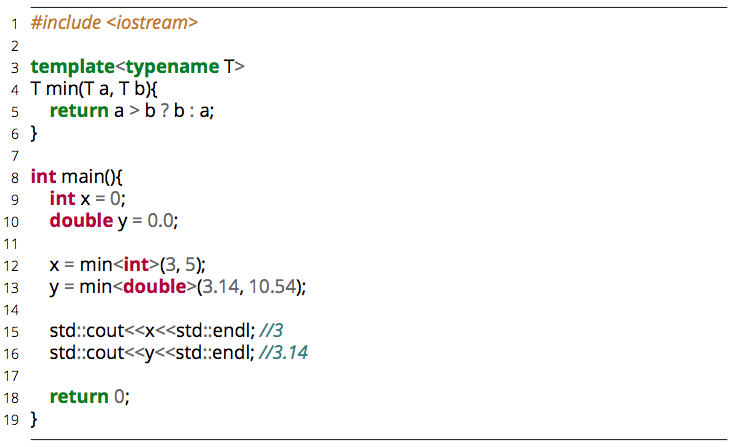
\includegraphics[height=60mm]{/Users/lalanne/MyCode/GitHubProjects/MetaTalk/figures/min_tmp.png}\hspace{5mm}
            };
        \end{tikzpicture}
    \end{center}
\end{frame}

\begin{frame}{Type Computations}
    \begin{center}
        \begin{tikzpicture}[]
            \node[] at (0mm,0mm){
                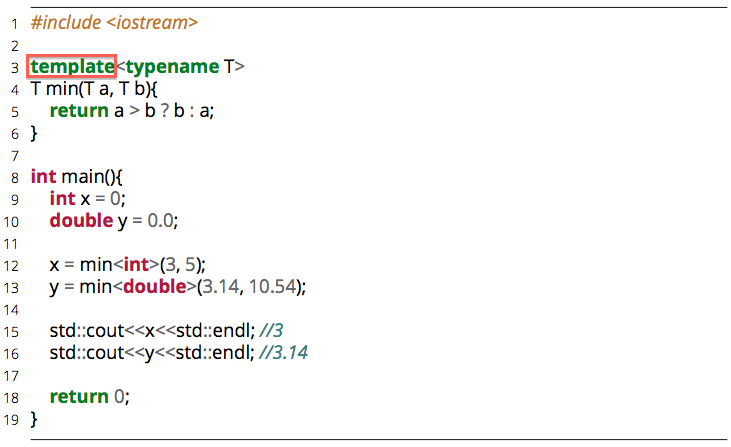
\includegraphics[height=60mm]{/Users/lalanne/MyCode/GitHubProjects/MetaTalk/figures/min_tmp_1.png}\hspace{5mm}
            };
        \end{tikzpicture}
    \end{center}
\end{frame}

\begin{frame}{Type Computations}
    \begin{center}
        \begin{tikzpicture}[]
            \node[] at (0mm,0mm){
                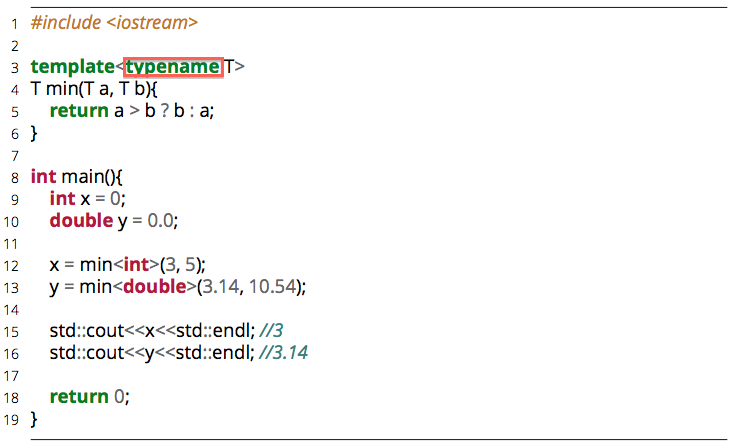
\includegraphics[height=60mm]{/Users/lalanne/MyCode/GitHubProjects/MetaTalk/figures/min_tmp_2.png}\hspace{5mm}
            };
        \end{tikzpicture}
    \end{center}
\end{frame}

\begin{frame}{Type Computations}
    \begin{center}
        \begin{tikzpicture}[]
            \node[] at (0mm,0mm){
                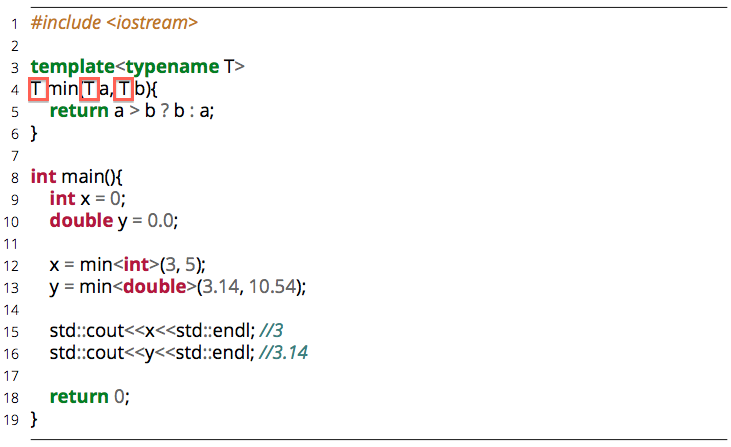
\includegraphics[height=60mm]{/Users/lalanne/MyCode/GitHubProjects/MetaTalk/figures/min_tmp_3.png}\hspace{5mm}
            };
        \end{tikzpicture}
    \end{center}
\end{frame}

\begin{frame}{Type Computations}
    \begin{center}
        \begin{tikzpicture}[]
            \node[] at (0mm,0mm){
                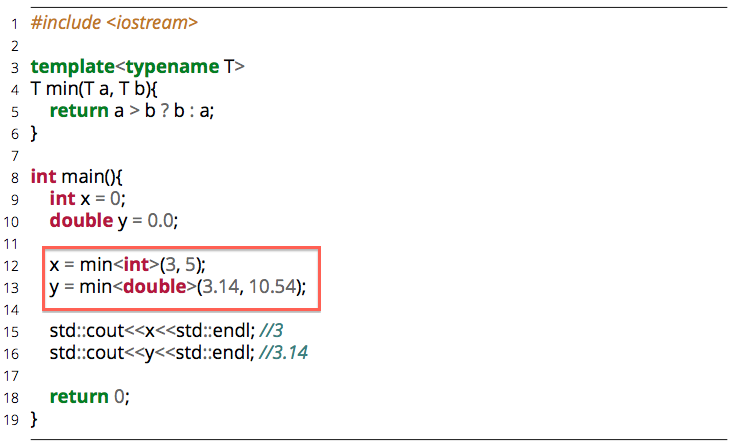
\includegraphics[height=60mm]{/Users/lalanne/MyCode/GitHubProjects/MetaTalk/figures/min_tmp_4.png}\hspace{5mm}
            };
        \end{tikzpicture}
    \end{center}
\end{frame}

\begin{frame}{Type Computations}
    \begin{center}
        \begin{tikzpicture}[]
            \node[] at (0mm,0mm){
                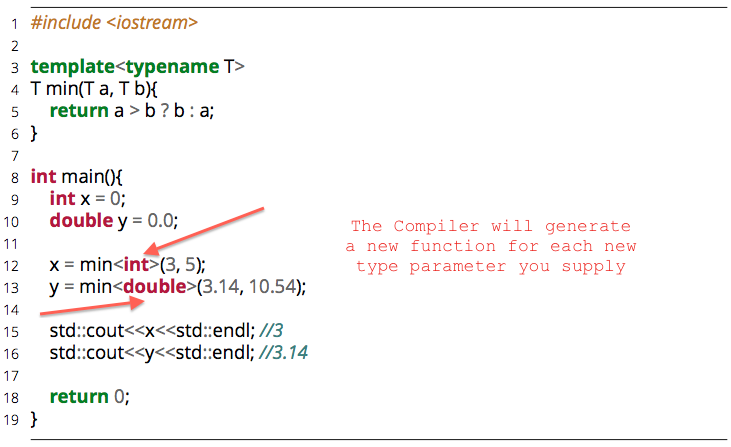
\includegraphics[height=60mm]{/Users/lalanne/MyCode/GitHubProjects/MetaTalk/figures/min_tmp_5.png}\hspace{5mm}
            };
        \end{tikzpicture}
    \end{center}
\end{frame}

\begin{frame}{Type Computations}
    \inputminted[mathescape,                                                       
        linenos,                                                           
        numbersep=5pt,                                                     
        frame=lines,                                                       
        bgcolor=White,                                                     
        fontsize=\scriptsize,                                              
        linenos,                                                           
        framesep=1.5mm]{c++}                                                 
        {/Users/lalanne/MyCode/GitHubProjects/MetaTalk/src/code/minmetatype_more.cpp}
\end{frame}

\begin{frame}{Type Computations}
    \begin{center}
        \begin{tikzpicture}[]
            \node[] at (0mm,0mm){
                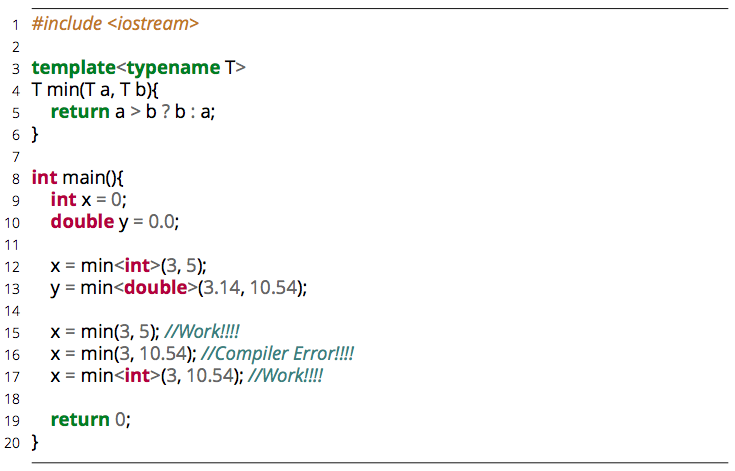
\includegraphics[height=60mm]{/Users/lalanne/MyCode/GitHubProjects/MetaTalk/figures/min_comp_types.png}\hspace{5mm}
            };
        \end{tikzpicture}
    \end{center}
\end{frame}

\begin{frame}{Type Computations}
    \begin{center}
        \begin{tikzpicture}[]
            \node[] at (0mm,0mm){
                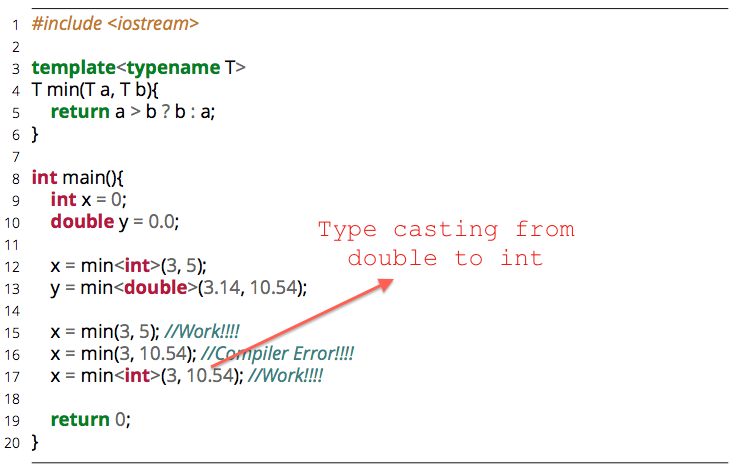
\includegraphics[height=60mm]{/Users/lalanne/MyCode/GitHubProjects/MetaTalk/figures/min_comp_types_1.png}\hspace{5mm}
            };
        \end{tikzpicture}
    \end{center}
\end{frame}

\begin{frame}[t]{Type Computations}
    \begin{itemize}
        \item New code is generated for each new type that the compiler encounters
        \item A template instance is only created once
        \item Multiple calls use the same object code created
    \end{itemize}
    \begin{center}
        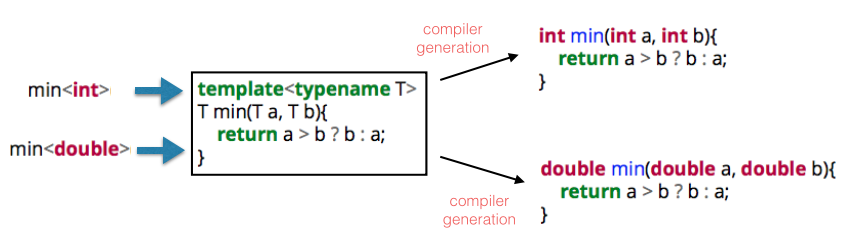
\includegraphics[height=30mm]{/Users/lalanne/MyCode/GitHubProjects/MetaTalk/figures/scheme.png}
    \end{center}
\end{frame}






